\section{Introduction}
\label{sec:intro}

Distributed training is an attractive solution to the problem of scaling deep
learning to training larger, more complex, and more accurate models. In short,
distributed training allows models to be trained across a cluster of machines
in a fraction of the time it would take to train on a single server. For
example, researchers at Facebook achieved near linear scalability when training
a ResNet-50 model on the ImageNet-1k dataset using 32 GPU-equipped
servers~\cite{goyal2017accurate}.

Distributed training is especially attractive for companies that want to
leverage cloud-based servers.  All major cloud providers---Google, Microsoft,
and Amazon---offer GPU server options to support deep learning.  However,
existing distributed training frameworks make traditional assumptions about the
lifetime of cloud servers in its cluster. Namely, that once a server is
acquired by the customer it will remain available until \emph{explicitly} released
back to the cloud provider by that customer. In this paper, we refer to such
servers as \emph{on-demand}. While this assumption is reasonable for many
deployments, we argue that it also represents a missed opportunity.   

In this work, we ask the question: what if we use \emph{transient} rather than
\emph{on-demand} servers for distributed training.  Transient servers offer
significantly lower costs than their on-demand equivalents with the added
complication that the cloud provider may \emph{revoke} them at any time---violating the
availability assumption discussed in the preceding paragraph.  Google,
Microsoft, and Amazon all offer transient servers, so the idea of 
distributed training with transient servers is applicable to all three major
cloud platforms.

Consider the following motivating experiment. Using a single on-demand GPU
server on Google Compute Engine, we were able to train a \emph{ResNet-32} model in 3.91 hours
with a total cost of \$2.83 on average (Table~\ref{intro:tbl:motivation}). When we use distributed training with
four on-demand servers---with each machine identical to the single server used 
the in previous runs---we improved the average training time to 0.99 hours
with similar overall cost of \$2.92. Finally, when we use distributed training
with four \emph{transient} servers we retain the improvement in training time,
1.05 hours on average, while significantly reducing the total cost to \$1.05 on
average (Figure~\ref{intro:motivation}). We saw these performance increases even though we made no significant
modifications to the distributed training framework and 13 of the 128 transient
servers (affecting 11 out of the 32 clusters) were revoked at some point prior
to the completion of training. We provide a more detailed analysis of this
experiment and the impact of server revocation in Section~\ref{sec:exp}.      

Our goal is to identify the important design considerations needed for
rearchitecting distributed training frameworks to support transient servers.
While the simple experiment above demonstrates the potential of distributed
training with transient servers (e.g., reduced training time and cost) as well
as the challenges (e.g., server revocation and availability), we believe that
transient servers also offer additional opportunities.  For example, price
dynamics make it more attractive to use clusters with machines drawn from
multiple, geographically-diverse, data centers. Such an approach raises
interesting questions about the impact of communication costs and latency on
training performance. Similarly, rather than use a cluster composed of servers 
of the same type,  we might employ heterogeneous clusters composed of machines
with different computational resources and capabilities. Finally, the clusters
themselves need not be static; instead, we might dynamically add or remove
servers to make distributed training more robust to server revocation or to
take advantage of volatile server pricing.   


\begin{table}[t]
\resizebox{\columnwidth}{!}{%
\begin{tabular}{@{}ccccc@{}}
\toprule
 &  & \cellcolor[HTML]{FFFFFF}{\color[HTML]{333333} \textbf{\begin{tabular}[c]{@{}c@{}}Training time \\ (hours)\end{tabular}}} & \cellcolor[HTML]{FFFFFF}{\color[HTML]{333333} \textbf{\begin{tabular}[c]{@{}c@{}}Cost\\ (\$)\end{tabular}}} & \cellcolor[HTML]{FFFFFF}{\color[HTML]{333333} \textbf{\begin{tabular}[c]{@{}c@{}}Accuracy\\ (\%)\end{tabular}}} \\ \midrule
\multicolumn{1}{c|}{} & \textit{4 K80 transient} & (1.05, 0.17) & (1.05, 0.02) & (91.23, 1.30) \\
\multicolumn{1}{c|}{} & \cellcolor[HTML]{EFEFEF}{\color[HTML]{000000} \textit{1 K80 on-demand}} & \cellcolor[HTML]{EFEFEF}{\color[HTML]{000000} (3.91, 0.03)} & \cellcolor[HTML]{EFEFEF}{\color[HTML]{000000} (2.83, 0.02)} & \cellcolor[HTML]{EFEFEF}{\color[HTML]{000000} (93.07, 0.002)} \\
\multicolumn{1}{c|}{\multirow{-3}{*}{\textbf{\begin{tabular}[c]{@{}c@{}}Training \\ Setup\end{tabular}}}} & \multicolumn{1}{l}{\textit{4 K80 on-demand}} & (0.99, 0.02) & (2.92, 0.05) & (91.20, 1.01) \\ \midrule
\multicolumn{1}{c|}{} & \textit{r = 0 (21 out of 32)} & (0.98, 0.01) & (1.04, 0.01) & (91.06, 1.43) \\
\multicolumn{1}{c|}{} & \textit{r = 1 (8 out of 32)} & (1.13, 0.12) & (1.07, 0.01) & (91.83, 0.90) \\
\multicolumn{1}{c|}{\multirow{-3}{*}{\textbf{\begin{tabular}[c]{@{}c@{}}Transient\\ revocation \\ scenarios\end{tabular}}}} & \textit{r = 2 (2 out of 32)} & (1.45, 0.50) & (1.10, 0.02) & (90.68, 0.30) \\ \bottomrule
\end{tabular}
}
\caption{\textbf{Benefits of transient distributed training.} On average,
  training with 4-\texttt{K80} transient GPU servers results in a 3.72X speedup with
  62.9\% monetary savings, compared to running on one K80 on-demand GPU server.
  In addition, we observe a 1.2\% drop in accuracy compared to single GPU
  server training. However, the slightly lower accuracy is due to training on
  stale model parameters in distributed asynchronous training. That is,
  training with 4-\texttt{K80} servers, regardless of transient or on-demand, produces models with almost identical accuracies. Here $\textit{r = x (y out of 32)}$ denotes that the revocation of $x$ workers happens in $y$ clusters. 
Performance metrics are represented in a tuple of average and standard deviation throughout the paper, unless otherwise specified.}
\label{intro:tbl:motivation}
\end{table}


We conduct the first \emph{large-scale} empirical measurement study that 
quantifies the training performance of deep learning models using cloud transient servers.  
Through our study, we make the following additional contributions: 
\begin{itemize}
%\item We conduct the first \emph{large-scale} empirical measurement study that quantifies the training performance of deep learning models using cloud transient servers. 
\item We compare the training time and cost of distributed training using transient servers to on-demand servers. We observe up to 7.7X training speedup and up to 62.9\% monetary savings
in our experiments  when compared to the single GPU baseline. 
%our empirical analysis identifies the significant performance improvements with speeding up deep learning by almost 8X with more than 60\% monetary savings. 
\item We quantify the revocation impacts of transient servers on training
  performance and identify the importance of larger cluster sizes and the need
    to redesign distributed training frameworks. In addition, our observations
    about model accuracy reveal additional opportunities for mitigating
    revocation impacts, such as the need for cloud providers to support \emph{selective} revocation. 
\item We also demonstrate the benefits and limitations of using heterogeneous servers in distributed training. In particular, our findings suggest a number of plausible transient-aware designs for deep learning frameworks, including the ability to train with dynamic cluster sizes, to better exploit these cheap transient servers. 
\end{itemize}


\begin{figure}[t]
\centering
    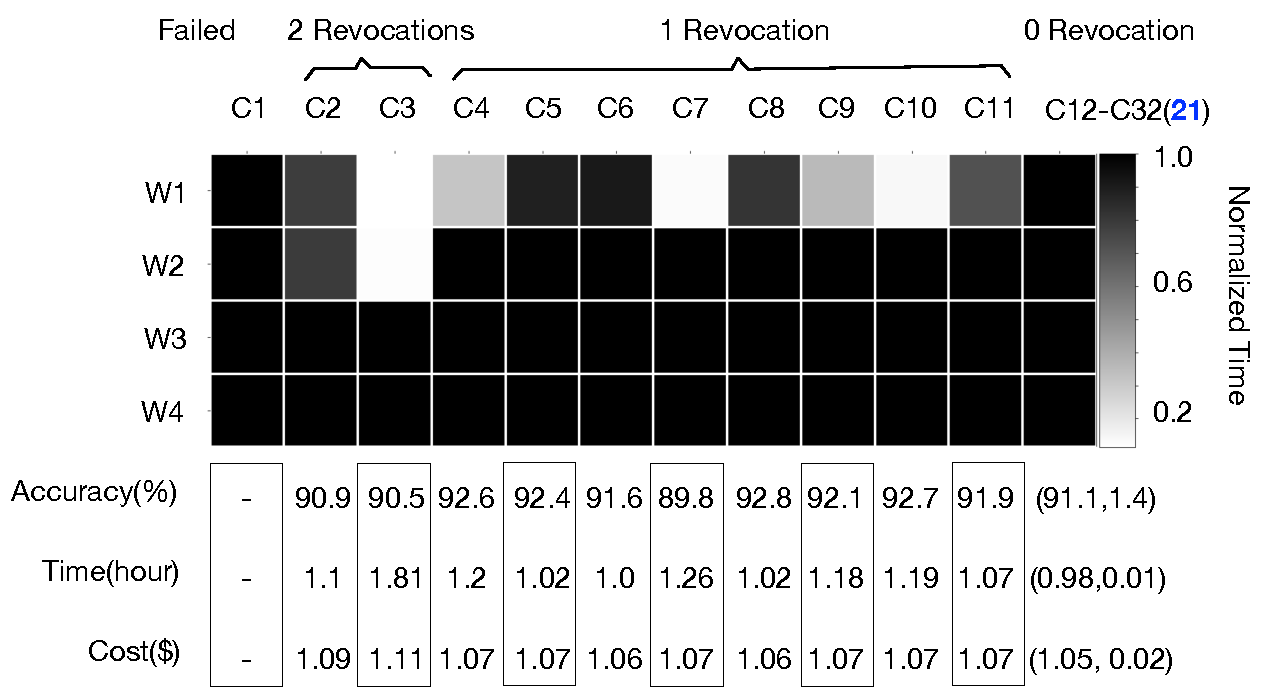
\includegraphics[width=\columnwidth ]{cluster_4_spots_heatmap.pdf}
\caption{\textbf{Quantifying distributed training performance using transient
  servers.} We launched \emph{32} transient GPU clusters for training the ResNet-32
  model on the Cifar-10 dataset. Each cluster $C_i$ was configured with four
  \texttt{K80} transient GPU servers ($W1$ to $W4$) and one parameter server.
  We observed that 21 out of 32 transient clusters completed training with 0
  revocations, and that 13 out of 128 \texttt{K80} transient servers were
  revoked during various training stages---the lighter the shade, the earlier
  the revocation. On average, training with 4 \texttt{K80} transient GPU
  servers resulted in a  3.72X speedup and 62.9\% monetary savings, compared to running on one \texttt{K80} on-demand GPU server.}  % 3.91 / 1.05 = 3.72X (time), (2.83-1.05) / 2.83 = 62.9% (cost)
%90\% of the transient servers and 65\% transient servers finish training without revocations, and achieve XX speedup with YY monetary savings compared running on single on-demand GPU server.}
    \label{intro:motivation}
\end{figure}
